   
\documentclass[11pt]{article}
\usepackage{amsmath,amsthm,verbatim,amssymb,amsfonts,amscd, graphicx}
\usepackage{graphicx}
\usepackage{float}
\topmargin0.0cm
\headheight0.0cm
\headsep0.0cm
\oddsidemargin0.0cm
\textheight23.0cm
\textwidth16.5cm
\footskip1.0cm
\theoremstyle{plain}
\newtheorem{theorem}{Theorem}
\newtheorem{corollary}{Corollary}
\newtheorem{lemma}{Lemma}
\newtheorem{proposition}{Proposition}
\newtheorem*{surfacecor}{Corollary 1}
\newtheorem{conjecture}{Conjecture} 
\newtheorem{question}{Question} 
\theoremstyle{definition}
\newtheorem{definition}{Definition}

\begin{document}
\title{CS 5220\\ Project 1 - Matrix Multiplication}
\author{Weici Hu(wh343)\\ Sheroze Sheriffdeen(mss385)\\ Qinyu Wang(qw78)}
\maketitle

\section{Overview}


In this project, we tried several methods to fine-tune square matrix multiplication.
Based on the \texttt{dgemm\_blocked.c}, we tried unrolling inner loop multiplication, modifying loop sequence to take advantage of SSE, experimenting with different optimization flags, multiple blocks sizes and copy optimizations. 

The next section reflects our various optimization attempts and their results. 

\section{Optimization Attempts}
\subsection{Block Multiplication with Multiple Block Sizes}
\subsubsection{Approach}
Working off of \texttt{dgemm\_blocked.c}, we tried different block sizes to examine the performance changes. 
\subsubsection{Results}
Figure \ref{pow_2_blocks} shows the performance of different approaches with various block sizes. (block sizes are a multiple of 2). The performance gain for varying block sizes is not immense but a block size of 64 performs better than other block sizes. \\

\begin{figure}[H]
    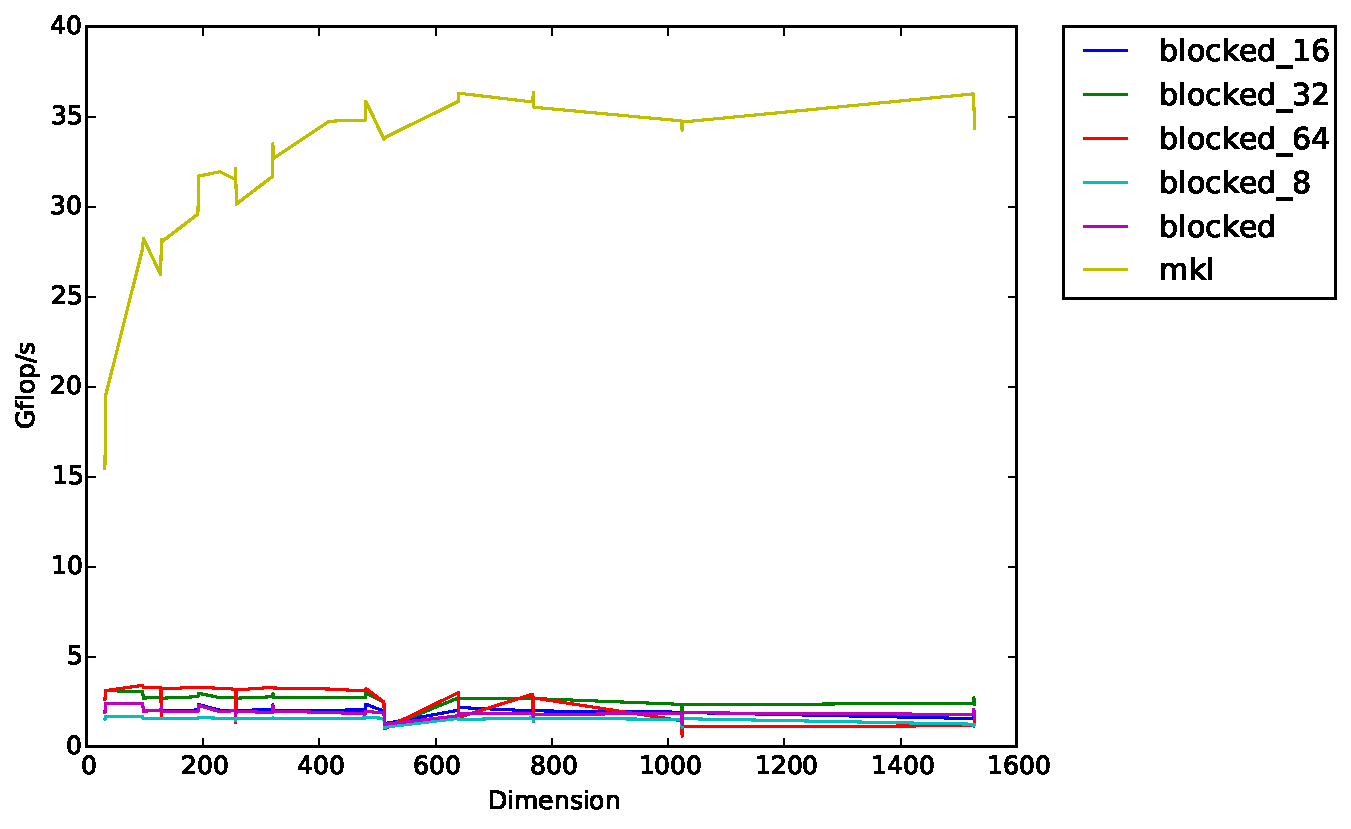
\includegraphics[width=0.9\textwidth]{timing_block_size_changes.pdf}
    \caption{Block size variation}
    \label{pow_2_blocks}
\end{figure} 

In addition, we attempted block sizes that are not a multiple of 2. Figure \ref{odd_blocks} is the comparison of the performance against a block size of 64.\\
\begin{figure}[H]
    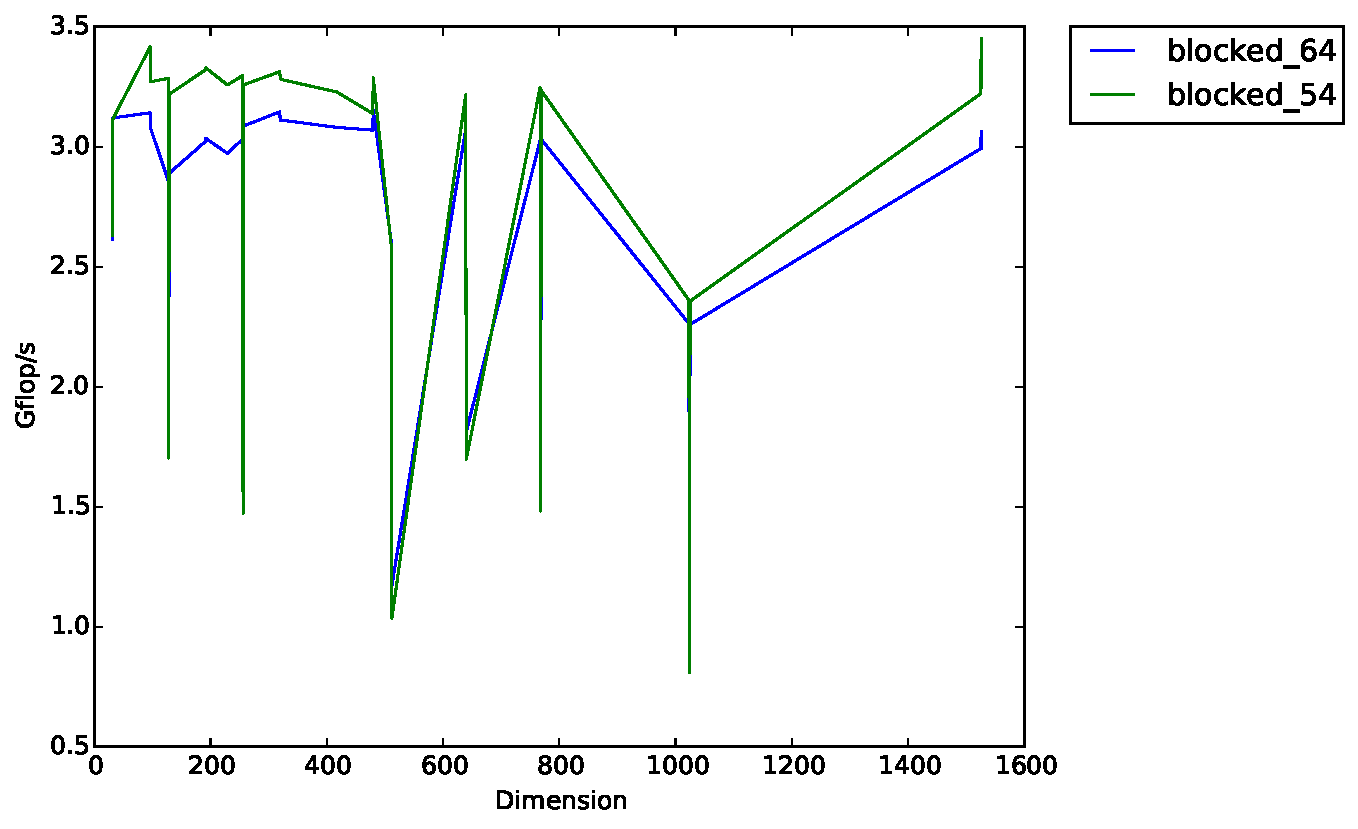
\includegraphics[width=0.9\textwidth]{timing_54_64.pdf}
    \caption{Block size variation}
    \label{odd_blocks}
\end{figure} 


\subsection{Block Multiplication with Manual Loop Unrolling}
\subsubsection{Approach}
In this approach, we manually unrolled 4 computations in the inner most loop of the matrix multiplication of a block. 
\subsubsection{Results}
Figure \ref{unrolled_vs_regular} compares the performance of the unrolled blocked version against the vanilla blocked approach. The unrolled versions clearly perform better than the original blocked approach but not by much. 
\begin{figure}[H]
    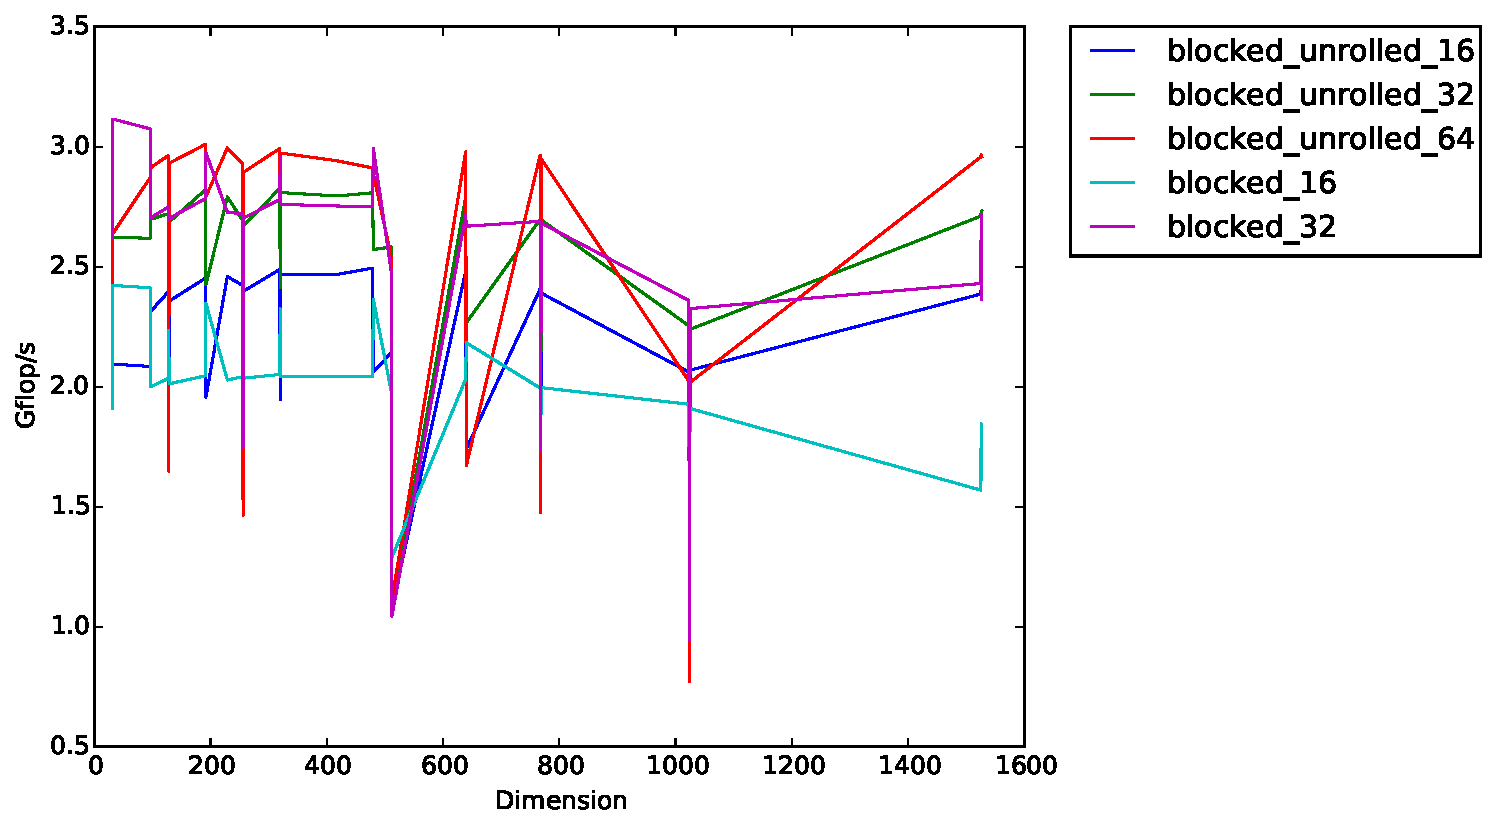
\includegraphics[width=0.9\textwidth]{timing_unrolled_vs_nonunrolled.pdf}
    \caption{Unrolled blocks vs regular blocks}
    \label{unrolled_vs_regular}
\end{figure} 

\subsection{Compiler Optimization Flags}
\subsubsection{Approach}
Using the blocked approach as a baseline, we examine the effect of various compiler flags on the multiplication.
\subsubsection{Results}
Figure \ref{all_optimized_blocked} shows the performance of blocked multiplication with the flags, \texttt{-O3 -march=native -funroll-loops}.
\begin{figure}[H]
    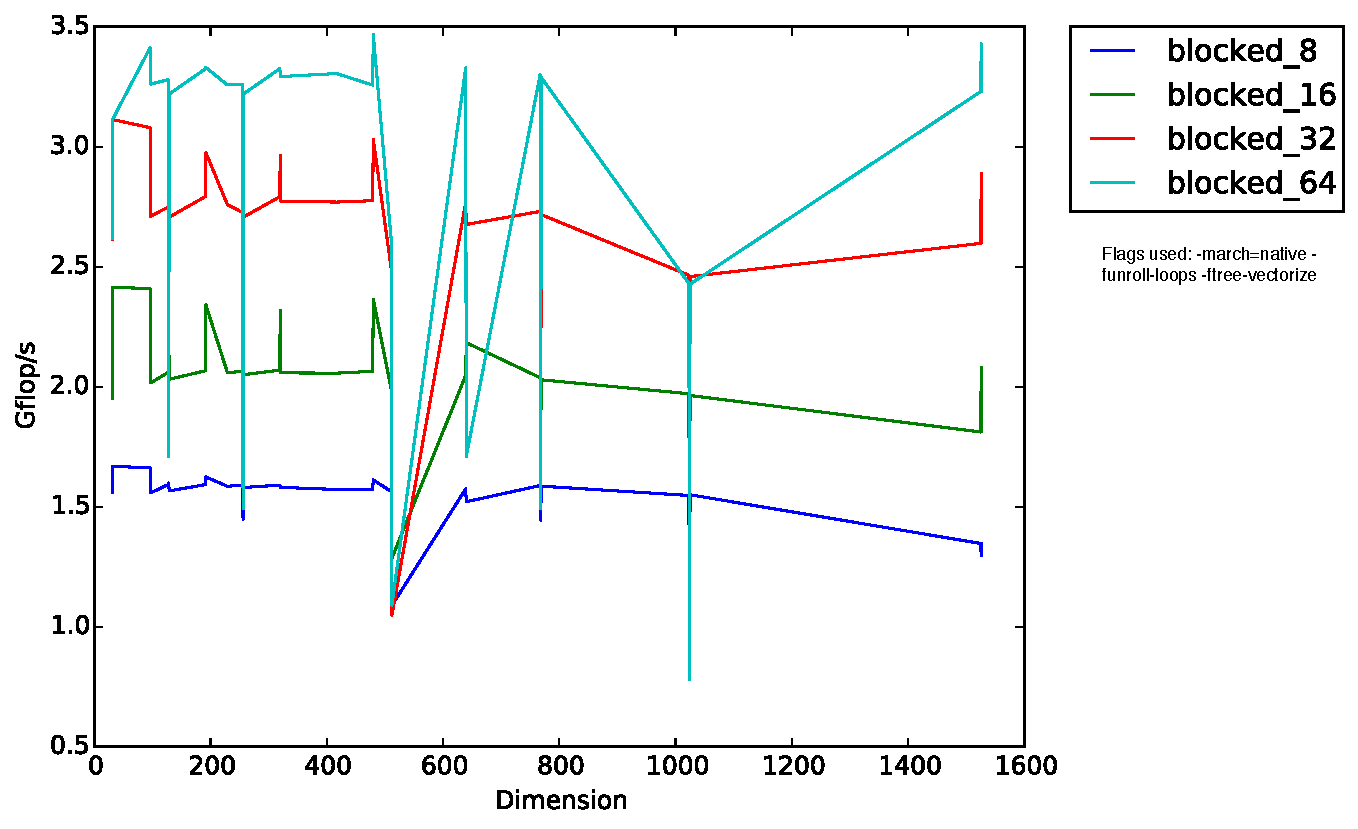
\includegraphics[width=0.9\textwidth]{timing_flags_blocked.pdf}
    \caption{Compiler flags \texttt{-O3 -march=native -funroll-loops}}
    \label{all_optimized_blocked}
\end{figure} 

Figure \ref{funroll_vanilla} shows the performance of blocked multiplication with the flags, \texttt{-O3 -funroll-loops} vs just \texttt{-O3}. It appears that merely having the \texttt{-O3} flag performs as well as having loops unrolled. 
\begin{figure}[H]
    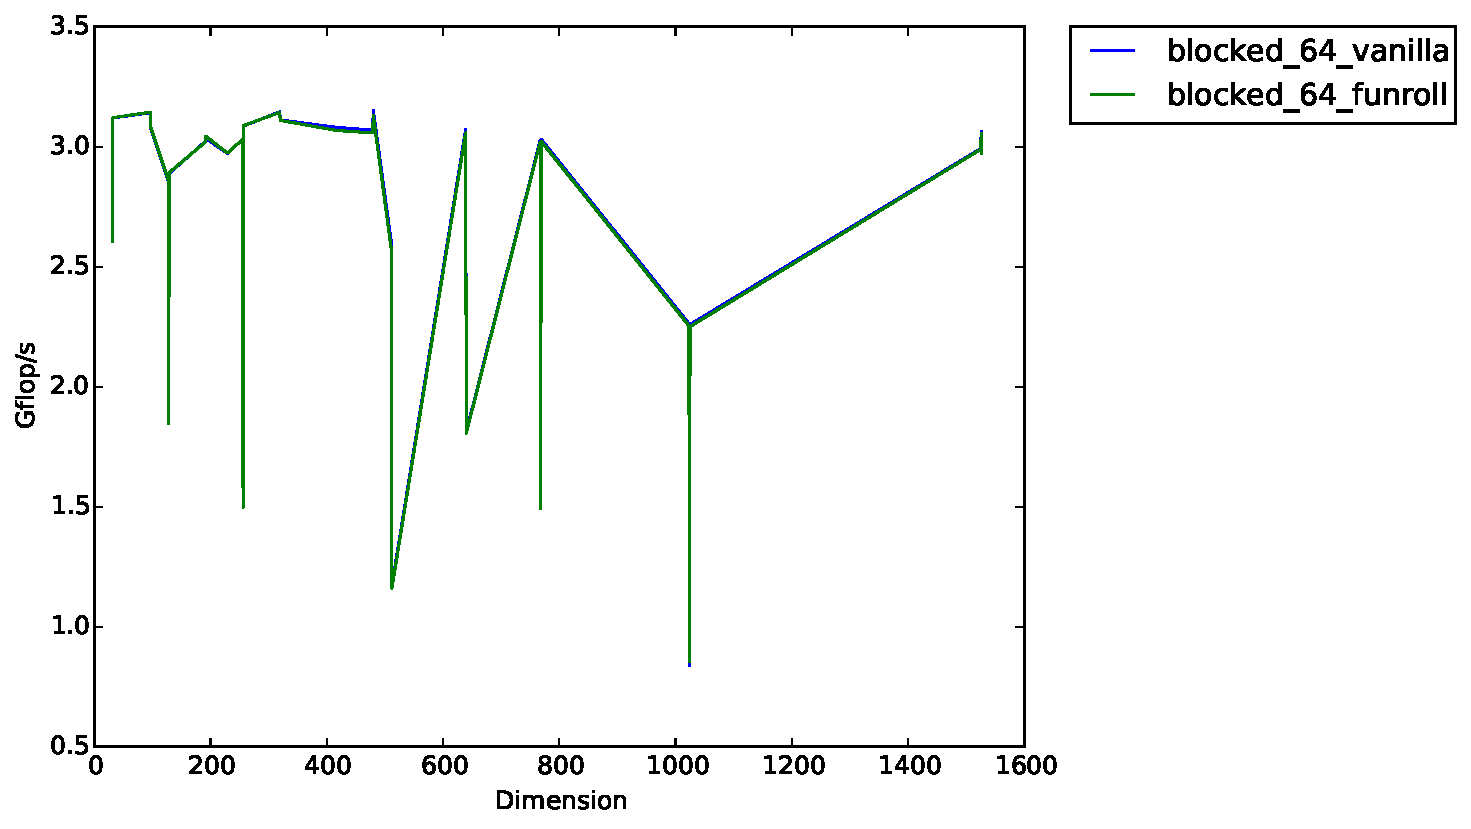
\includegraphics[width=0.9\textwidth]{timing_funroll_vanilla.pdf}
    \caption{Compiler flags \texttt{-O3 -funroll-loops}}
    \label{funroll_vanilla}
\end{figure} 


\subsection{Loop reordering}
\subsubsection{Approach}
The current block multiplication in the innermost loop does not have unit stride with $i, j, k$ loop ordering. 
\subsubsection{Results}

\begin{figure}[H]
    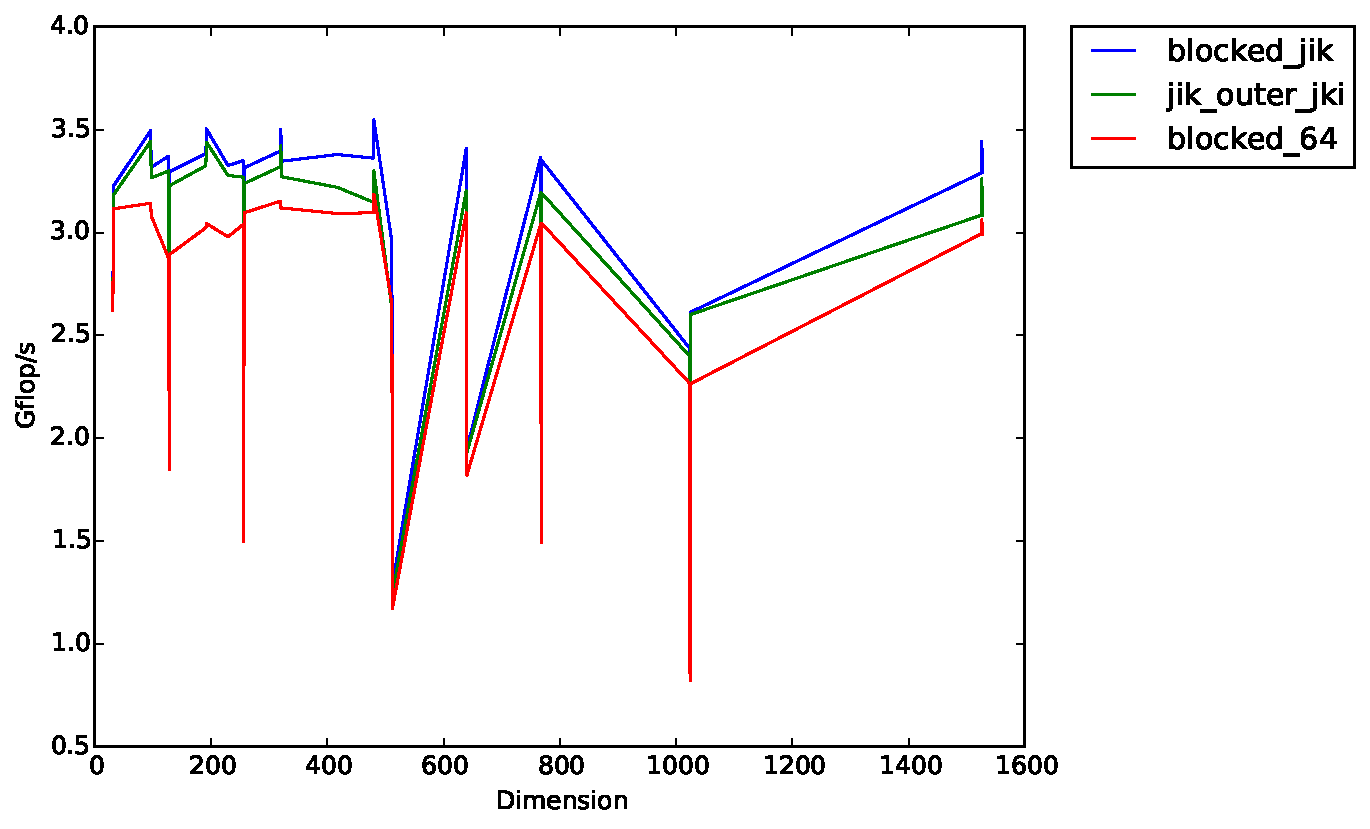
\includegraphics[width=0.9\textwidth]{timing_loop_reorder_fast.pdf}
    \caption{Loop reordering \texttt{ijk} vs \texttt{jik} vs \texttt{jik} and outer loop \texttt{jki}}
    \label{basic_copy_opt}
\end{figure} 

\subsection{Copy Optimization}
\subsubsection{Approach}
In the basic version of dgemm, we see drops near matrix sizes that are a multiple of 2. This is caused by conflict misses due to associative caches. To prevent this, we attempted a copy optimization over the basic dgemm implementation.
\subsubsection{Results}
There is a clear improvement in performance and the conflict misses are converted to gains in performance as seen in Figure \ref{basic_copy_opt}. Copy optimization is clearly a step in the right direction.
\begin{figure}[H]
    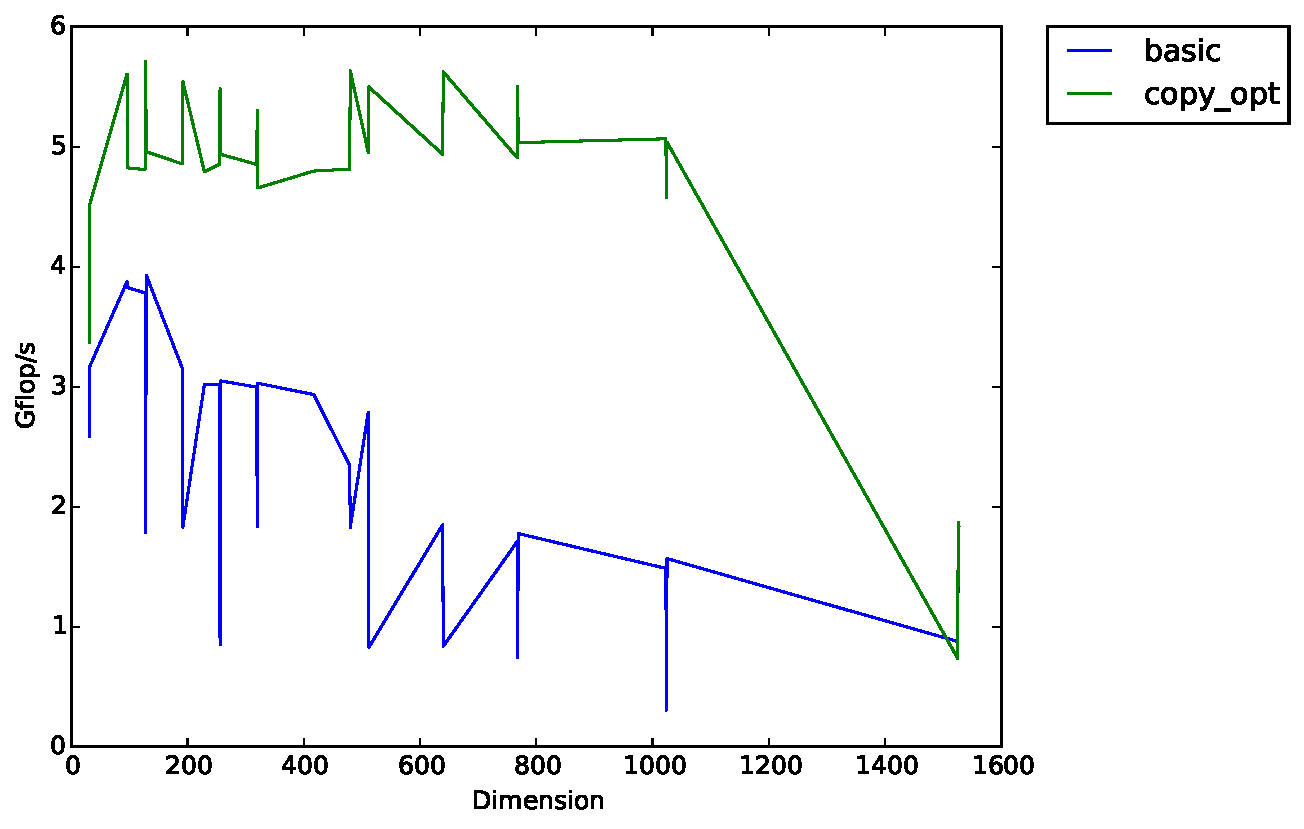
\includegraphics[width=0.9\textwidth]{timing_basic_vs_copy_opt.pdf}
    \caption{Basic DGEMM vs DGEMM with Copy Optimization}
    \label{basic_copy_opt}
\end{figure} 
\subsection{Compiler flags on Copy Optimization}
\subsubsection{Approach}
We use \texttt{-03} and \texttt{-02} optimization flags when we compile the copy optimization code.
\subsubsection{result}
\texttt{-02} optimizer is performing better than \texttt{-03}  especially when the size of the matrix grows larger.
\begin{figure}[H]
    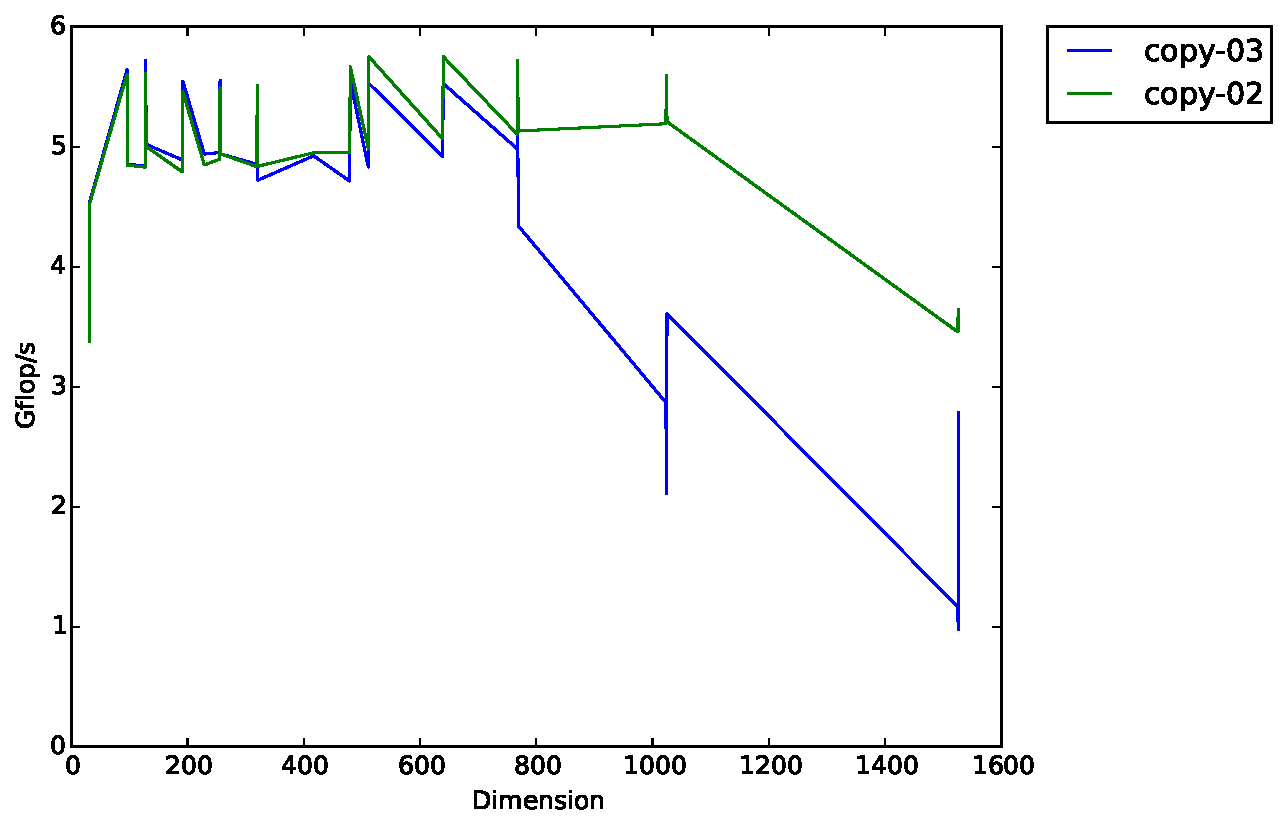
\includegraphics[width=0.9\textwidth]{timing_flag0203_copy.pdf}
    \caption{-03 vx -02 on Copy Optimization}
    \label{0203}
\end{figure}
 

\subsection{Restrict Keyword}

\subsubsection{Approach}
Telling the compiler that our matrix pointers will not be aliasing is another approach suggested on the writeup. 
\subsubsection{Results}

Figure \ref{basic_restrict} shows the performance difference between the basic DGEMM implementation and the DGEMM implementation with the \texttt{restrict keyword}. \texttt{restrict} keyword provides good performance benefits. There is a caveat here since we assumed that the pointer \texttt{A} and \texttt{B} passed to \texttt{square\_dgemm} will not alias. 

\begin{figure}[H]
    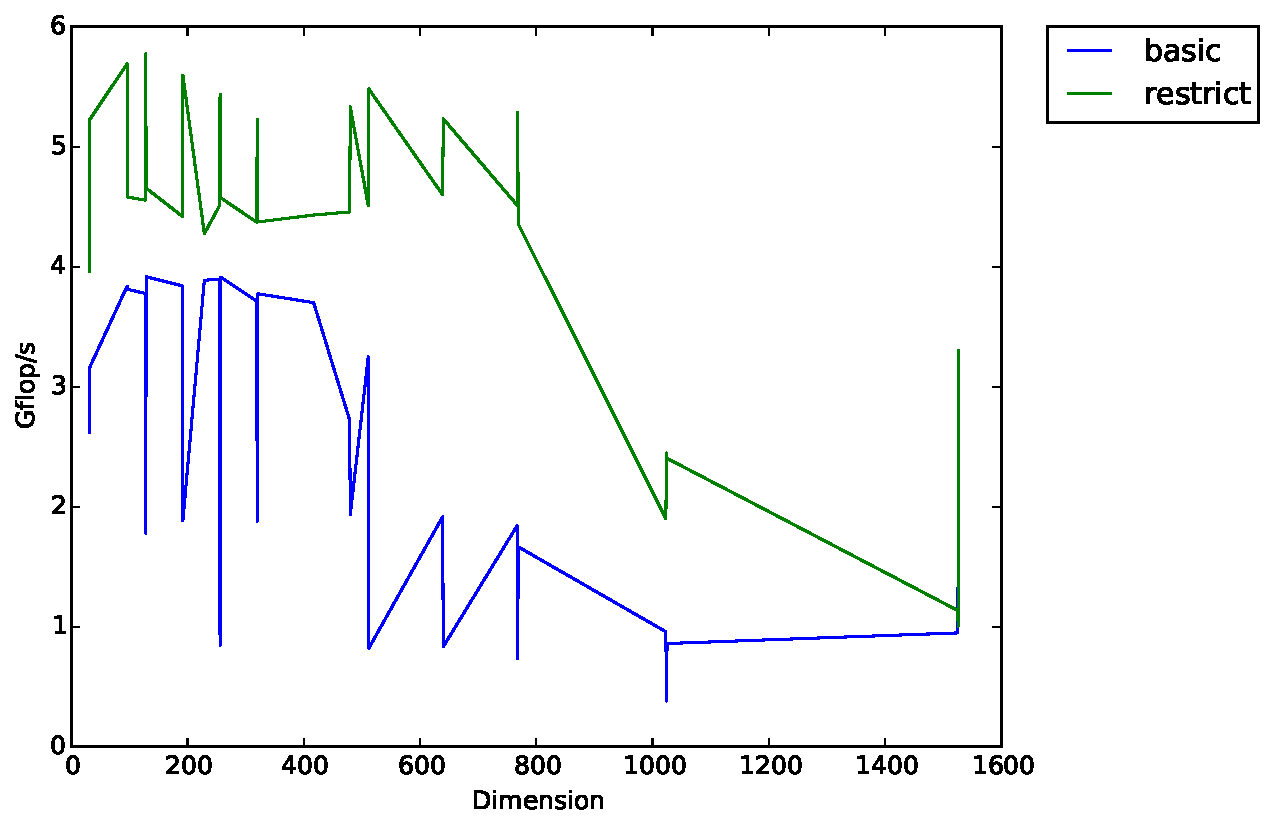
\includegraphics[width=0.9\textwidth]{timing_basic_vs_restrict.pdf}
    \caption{Basic DGEMM vs DGEMM with \texttt{restrict} keyword}
    \label{basic_restrict}
\end{figure} 

To eliminate the aliasing assumption, we intended to couple the \texttt{restrict} keyword and copy optimization to provide a stronger guarantee of not aliasing. The result as shown in figure \ref{restrict_copy_opt} shows that the performance decreases. This may be due to incorrect implementation of the restrict keyword in our code. 

\begin{figure}[H]
    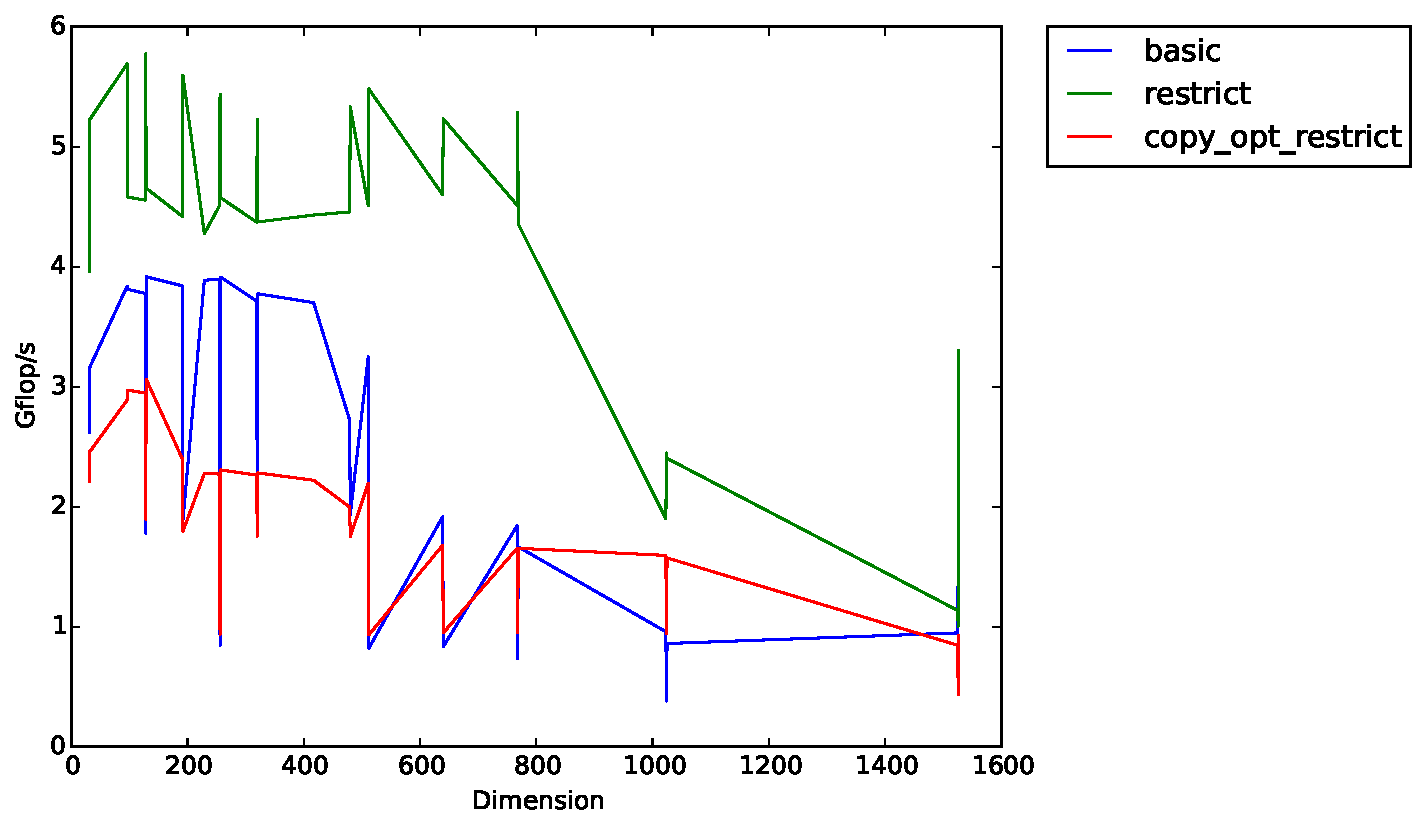
\includegraphics[width=0.9\textwidth]{timing_copy_opt_restrict.pdf}
    \caption{Basic DGEMM vs DGEMM with \texttt{restrict} keyword}
    \label{restrict_copy_opt}
\end{figure} 
\section{Next Steps}

\subsection{AVX Instructions}
We want to try AVX instructions to take advantage of using multiple registers at once. However we find that there are still bugs in our code and it is difficult to debug on the cluster machines. So we are currently configuring the Intel icc and Parallel Studio on our own laptop.

\subsection{Copy Optimization with Blocks}
We are also interested in combine copy optimization with block implementation. As shown above, we have implemented the copy optimization on the basic implementation, and when the matrix becomes too big the copy optimization fails. We believe by using the block implementation, we can avoid the performance drop.

\subsection{Autotuning}
Furthermore, we are interested in automating much of the block size search process once the memory layout and copy optimization ideas are fleshed out. 



 
 
\end{document}